\documentclass[aspectratio=169,9pt]{beamer}

% Theme
\usetheme{Madrid}
\usecolortheme{seahorse}

% Packages
\usepackage[utf8]{inputenc}
\usepackage[T1]{fontenc}
\usepackage{graphicx}
\usepackage{booktabs}
\usepackage{tikz}
\usepackage{xcolor}
\usepackage{fontawesome5}

% Smaller fonts for items
\setbeamerfont{itemize/enumerate body}{size=\small}
\setbeamerfont{itemize/enumerate subbody}{size=\footnotesize}
\setbeamerfont{block body}{size=\small}
\setbeamerfont{block title}{size=\normalsize}

% Custom colors
\definecolor{revoBlue}{RGB}{52, 152, 219}
\definecolor{revoRed}{RGB}{231, 76, 60}
\definecolor{revoGreen}{RGB}{39, 174, 96}
\definecolor{revoDark}{RGB}{44, 62, 80}
\definecolor{revoOrange}{RGB}{230, 126, 34}

\setbeamercolor{frametitle}{bg=revoDark,fg=white}
\setbeamercolor{title}{bg=revoDark,fg=white}
\setbeamercolor{structure}{fg=revoBlue}
\setbeamercolor{block title}{bg=revoBlue,fg=white}
\setbeamercolor{block body}{bg=revoBlue!10}

% Title
\title[\textbf{Helicopter vs Car Analysis}]{\textbf{Helicopter vs Car Travel Time Analysis}}
\subtitle{A Comprehensive Comparison of Traffic Scenarios\\New York \& Los Angeles}
\author{REVO Helicopter Services}
\institute{Strategic Analysis Division}
\date{December 2025}

\begin{document}

% ============================================================================
% TITLE SLIDE
% ============================================================================
\begin{frame}
\titlepage
\end{frame}

% ============================================================================
% AGENDA
% ============================================================================
\begin{frame}{Agenda}
\tableofcontents
\end{frame}

% ============================================================================
\section{Introduction}
% ============================================================================

\begin{frame}{The Problem: Urban Traffic Congestion}
\begin{columns}
\column{0.5\textwidth}
\begin{block}{The Challenge}
\begin{itemize}
    \item Business travelers need reliable airport access
    \item Traffic is unpredictable and often severe
    \item Missing flights = significant business impact
    \item Stress and time loss affect productivity
\end{itemize}
\end{block}

\column{0.5\textwidth}
\begin{alertblock}{Worst Case Reality}
\begin{center}
\textbf{During severe traffic:}\\[0.3em]
\large{\textcolor{revoRed}{4.68x}} \small{travel time}\\[0.3em]
\large{\textcolor{revoRed}{12 km/h}} \small{average speed}\\[0.3em]
\footnotesize{\textit{(barely faster than walking!)}}
\end{center}
\end{alertblock}
\end{columns}
\end{frame}

\begin{frame}{Study Overview}
\begin{columns}
\column{0.6\textwidth}
\begin{block}{Scope}
\begin{itemize}
    \item \textbf{New York}: 70 wealthy ZIP codes $\rightarrow$ JFK
    \item \textbf{Los Angeles}: 44 wealthy ZIP codes $\rightarrow$ LAX
    \item \textbf{Data}: Google Traffic (Pessimistic)
    \item \textbf{Routing}: OSRM + FAA Helipad Data
\end{itemize}
\end{block}

\column{0.4\textwidth}
\begin{exampleblock}{Key Numbers}
\begin{center}
\large{114} \small{ZIP Codes}\\[0.2em]
\large{65} \small{Heliports}\\[0.2em]
\large{4} \small{Traffic Scenarios}\\[0.2em]
\large{27} \small{Manhattan ZIPs}
\end{center}
\end{exampleblock}
\end{columns}
\end{frame}

% ============================================================================
\section{Methodology}
% ============================================================================

\begin{frame}{Traffic Multipliers Explained}
\begin{center}
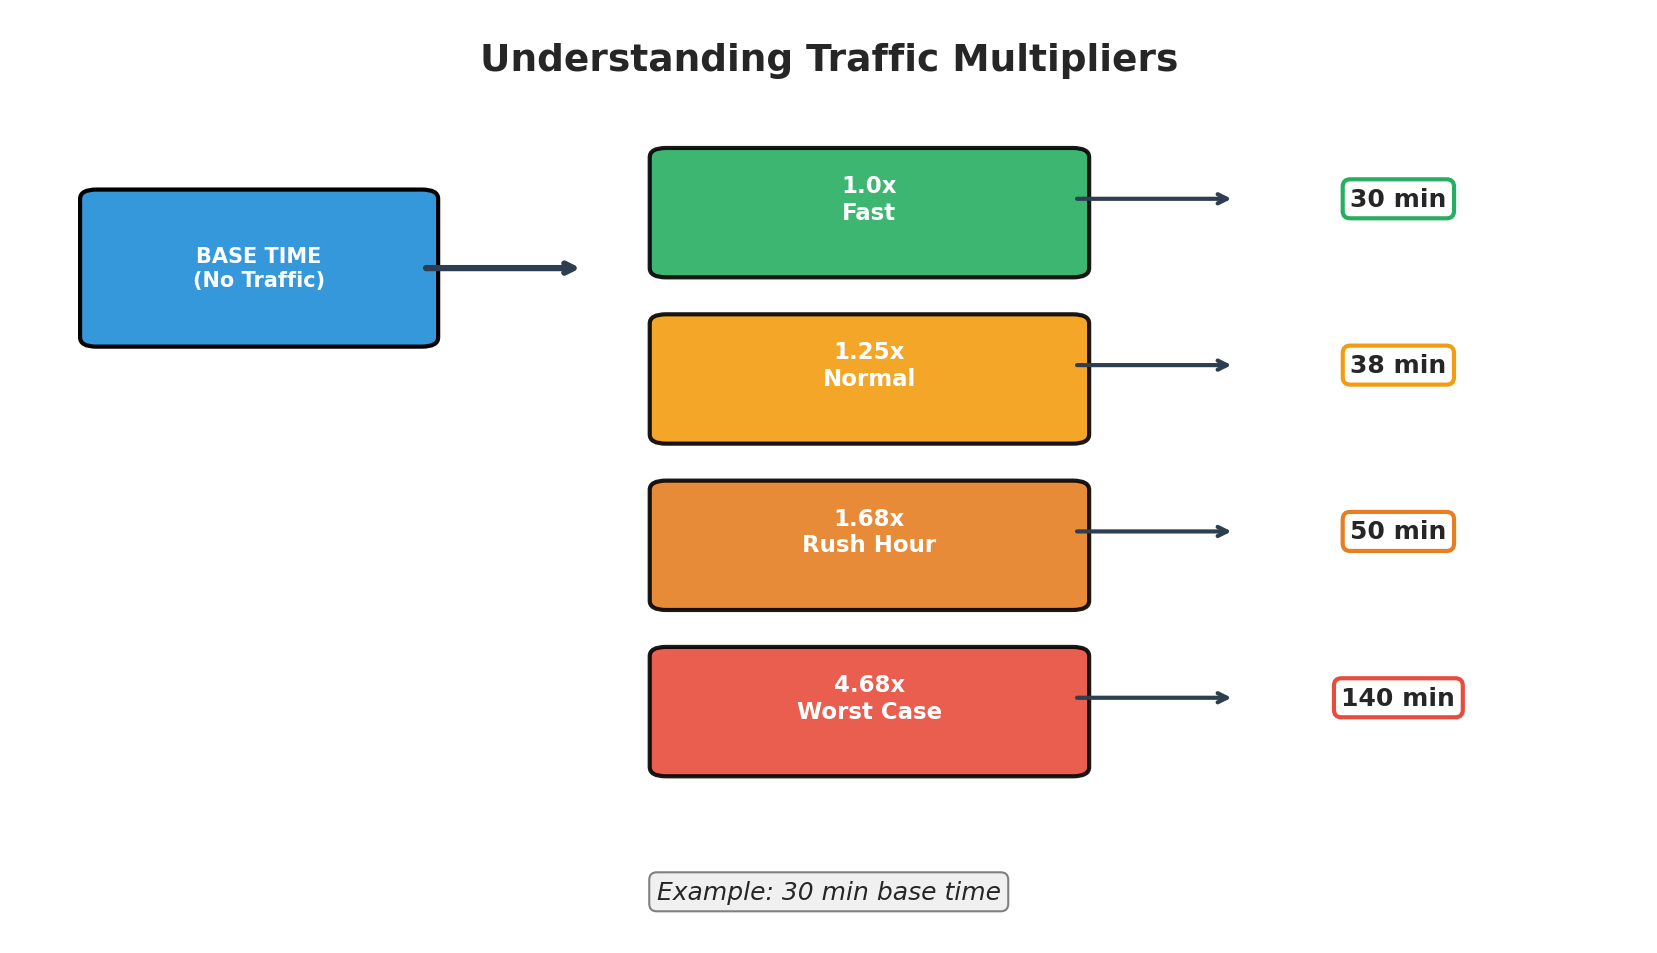
\includegraphics[width=0.7\textwidth,height=0.75\textheight,keepaspectratio]{../diagrams/traffic_multiplier_en.png}
\end{center}
\end{frame}

\begin{frame}{Journey Comparison: Car vs Helicopter}
\begin{center}
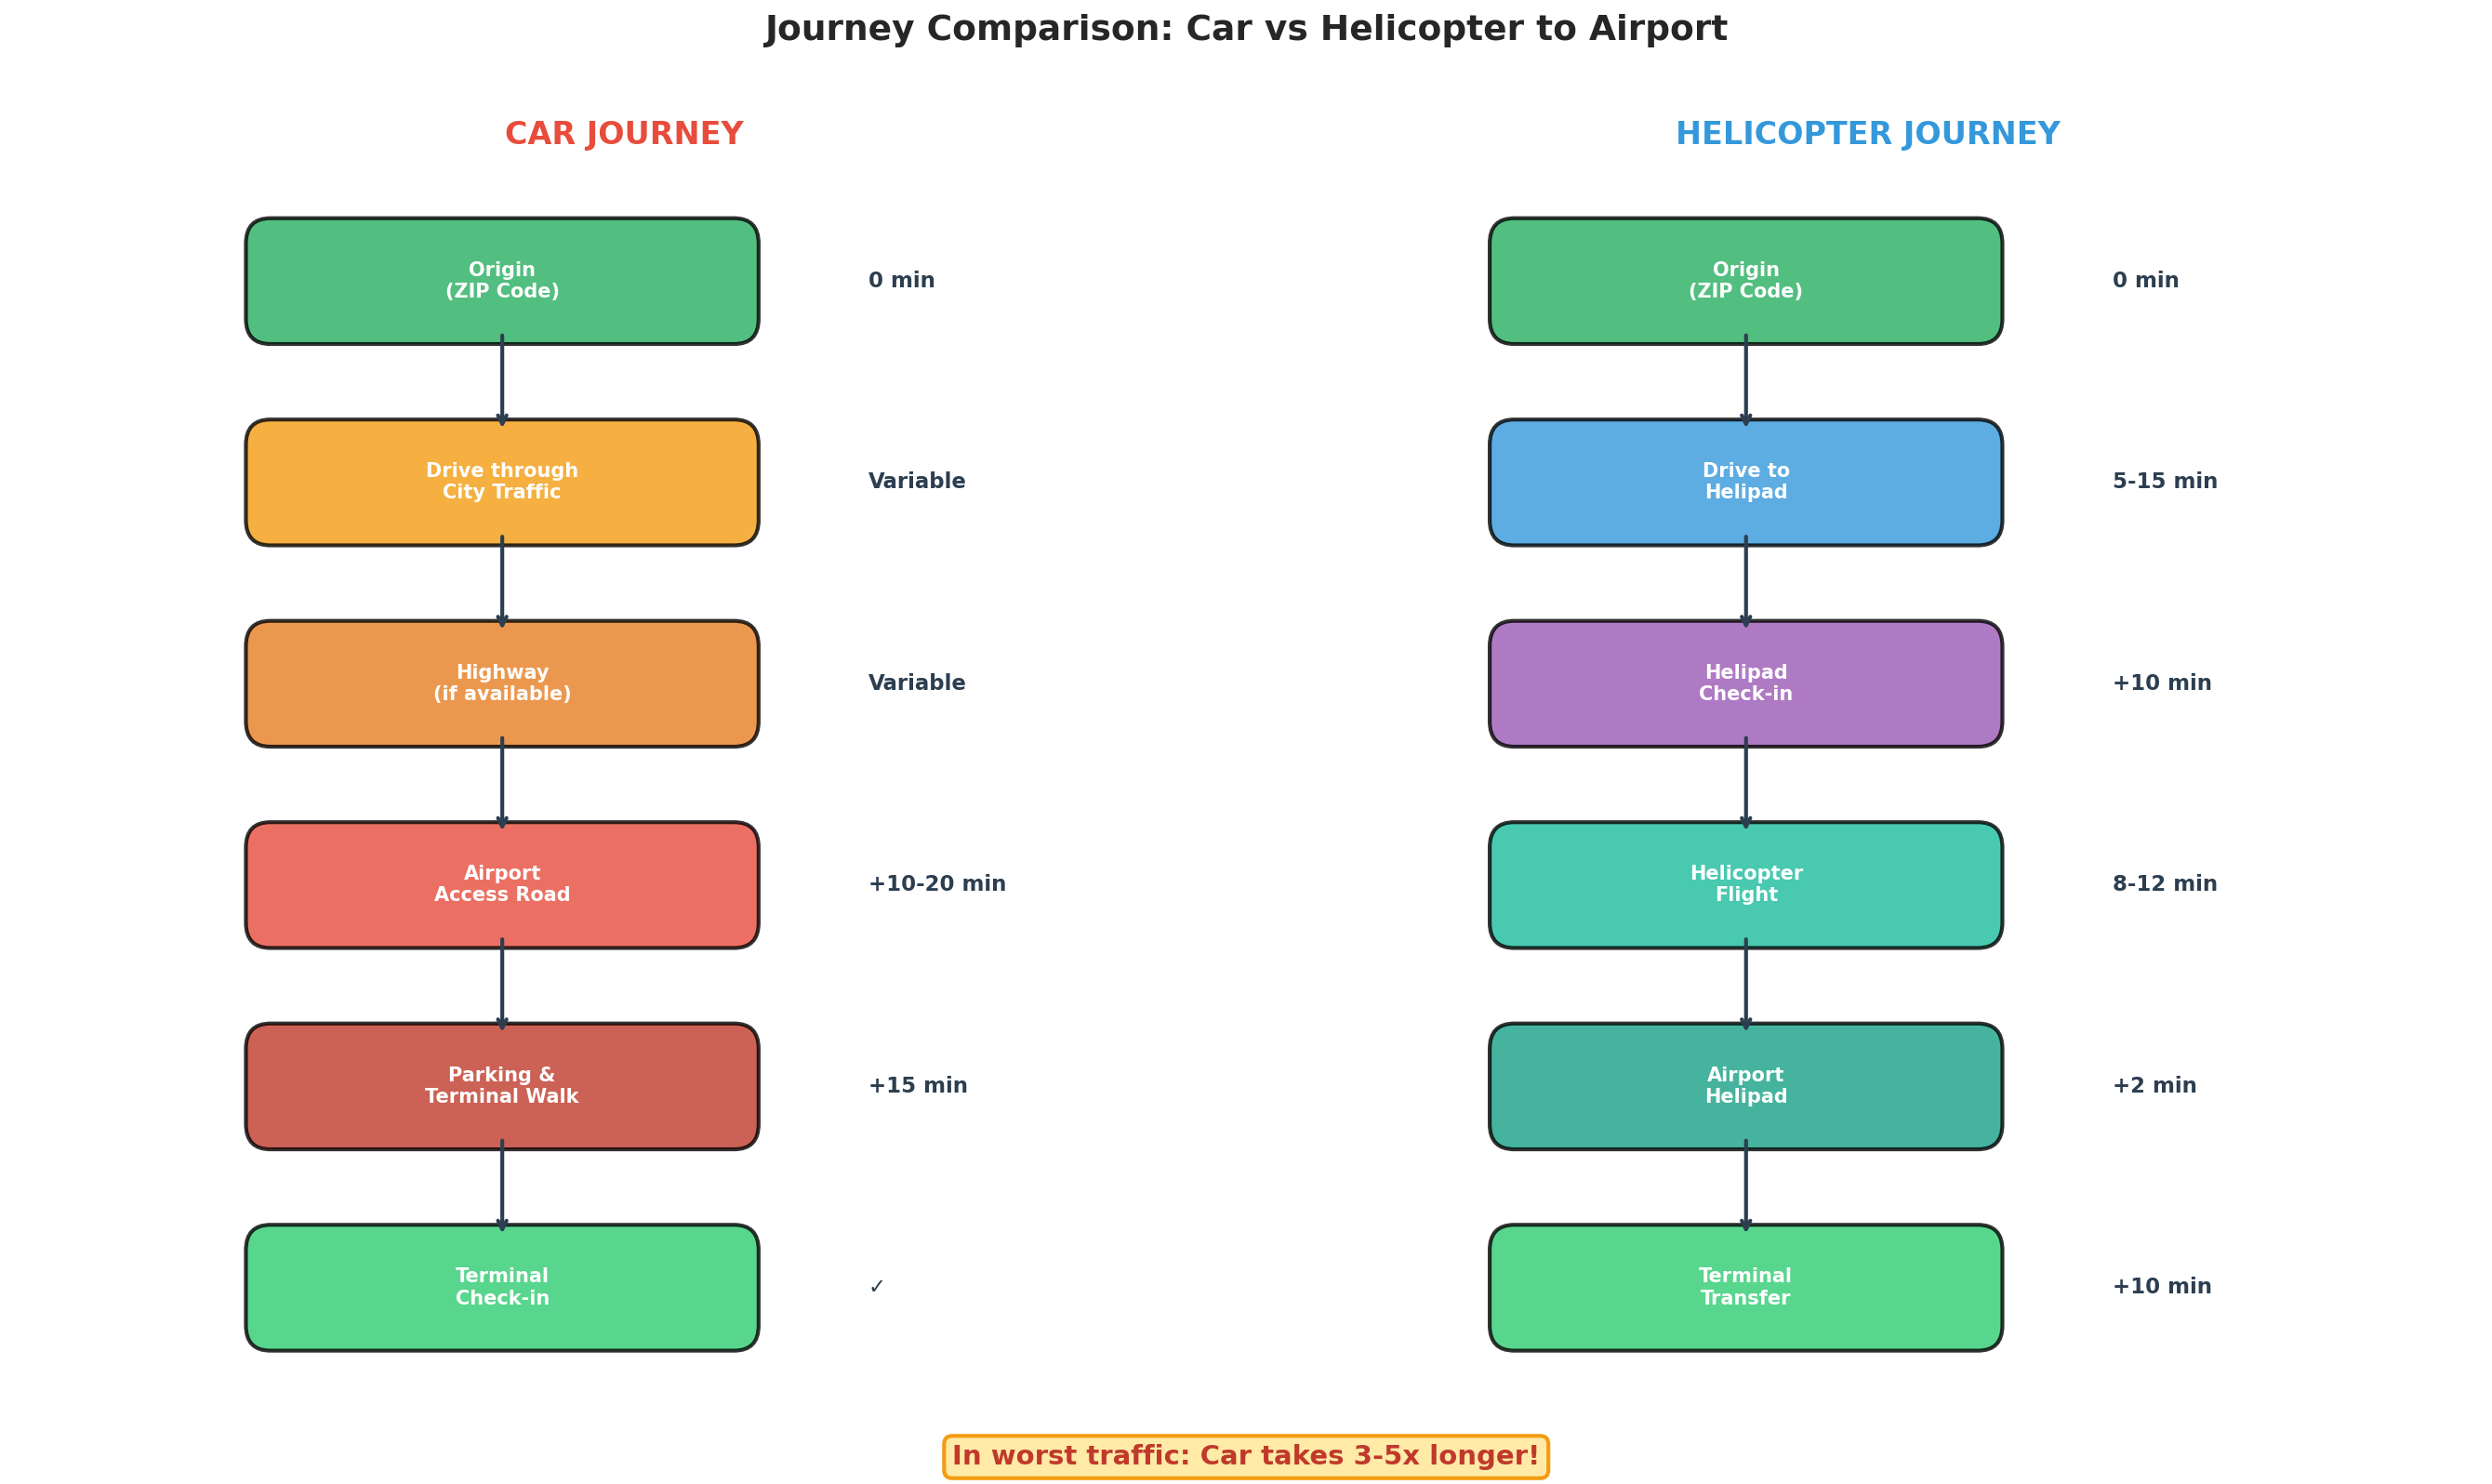
\includegraphics[width=0.85\textwidth,height=0.78\textheight,keepaspectratio]{../diagrams/journey_diagram_en.png}
\end{center}
\end{frame}

\begin{frame}{Helicopter Journey Components}
\begin{columns}
\column{0.5\textwidth}
\begin{block}{\faCarSide\ Step 1: Drive to Helipad}
\begin{itemize}
    \item Affected by traffic
    \item Manhattan helipad priority
    \item Average: 5-15 minutes
\end{itemize}
\end{block}

\begin{block}{\faHelicopter\ Step 3: Flight}
\begin{itemize}
    \item 200 km/h cruise speed
    \item Direct route
    \item 8-12 minutes typical
\end{itemize}
\end{block}

\column{0.5\textwidth}
\begin{block}{\faClipboardCheck\ Step 2: Check-in}
\begin{itemize}
    \item Fixed 10 minutes
    \item Security screening
    \item Boarding preparation
\end{itemize}
\end{block}

\begin{block}{\faWalking\ Step 4: Terminal Transfer}
\begin{itemize}
    \item Fixed 10 minutes
    \item Helipad to terminal
    \item Internal transport
\end{itemize}
\end{block}
\end{columns}
\end{frame}

\begin{frame}{Manhattan Helipad Network}
\begin{columns}
\column{0.5\textwidth}
\begin{block}{Approved Heliports}
\begin{itemize}
    \item \textbf{JRB}: Downtown/Wall St
    \item \textbf{JRA}: West 30th Street
    \item \textbf{6N5}: East 34th Street
    \item \textbf{3NY2}: Astoria (Queens)
\end{itemize}
\end{block}

\begin{alertblock}{Exclusions}
\faTimesCircle\ Police Heliports\\
\faTimesCircle\ One Police Plaza\\
\faTimesCircle\ Newport Beach Police (LA)
\end{alertblock}

\column{0.5\textwidth}
\begin{center}
\textbf{Why Manhattan-Only?}\\[0.5em]
\begin{tikzpicture}[scale=0.7]
    \draw[thick, fill=revoBlue!20] (0,0) rectangle (2,3.5);
    \node at (1,3) {\footnotesize Manhattan};
    \draw[ultra thick, revoRed] (2,1.75) -- (4,1.75);
    \node[revoRed] at (3,2.2) {\footnotesize \faTimesCircle\ Bridges};
    \node[revoRed] at (3,1.3) {\footnotesize \faTimesCircle\ Tunnels};
    \draw[thick, fill=gray!20] (4,0) rectangle (6,3.5);
    \node at (5,1.75) {\footnotesize NJ/Queens};
\end{tikzpicture}\\[0.5em]
\footnotesize{\textit{Avoid congested crossings!}}
\end{center}
\end{columns}
\end{frame}

% ============================================================================
\section{Results}
% ============================================================================

\begin{frame}{Scenario Comparison Overview}
\begin{center}
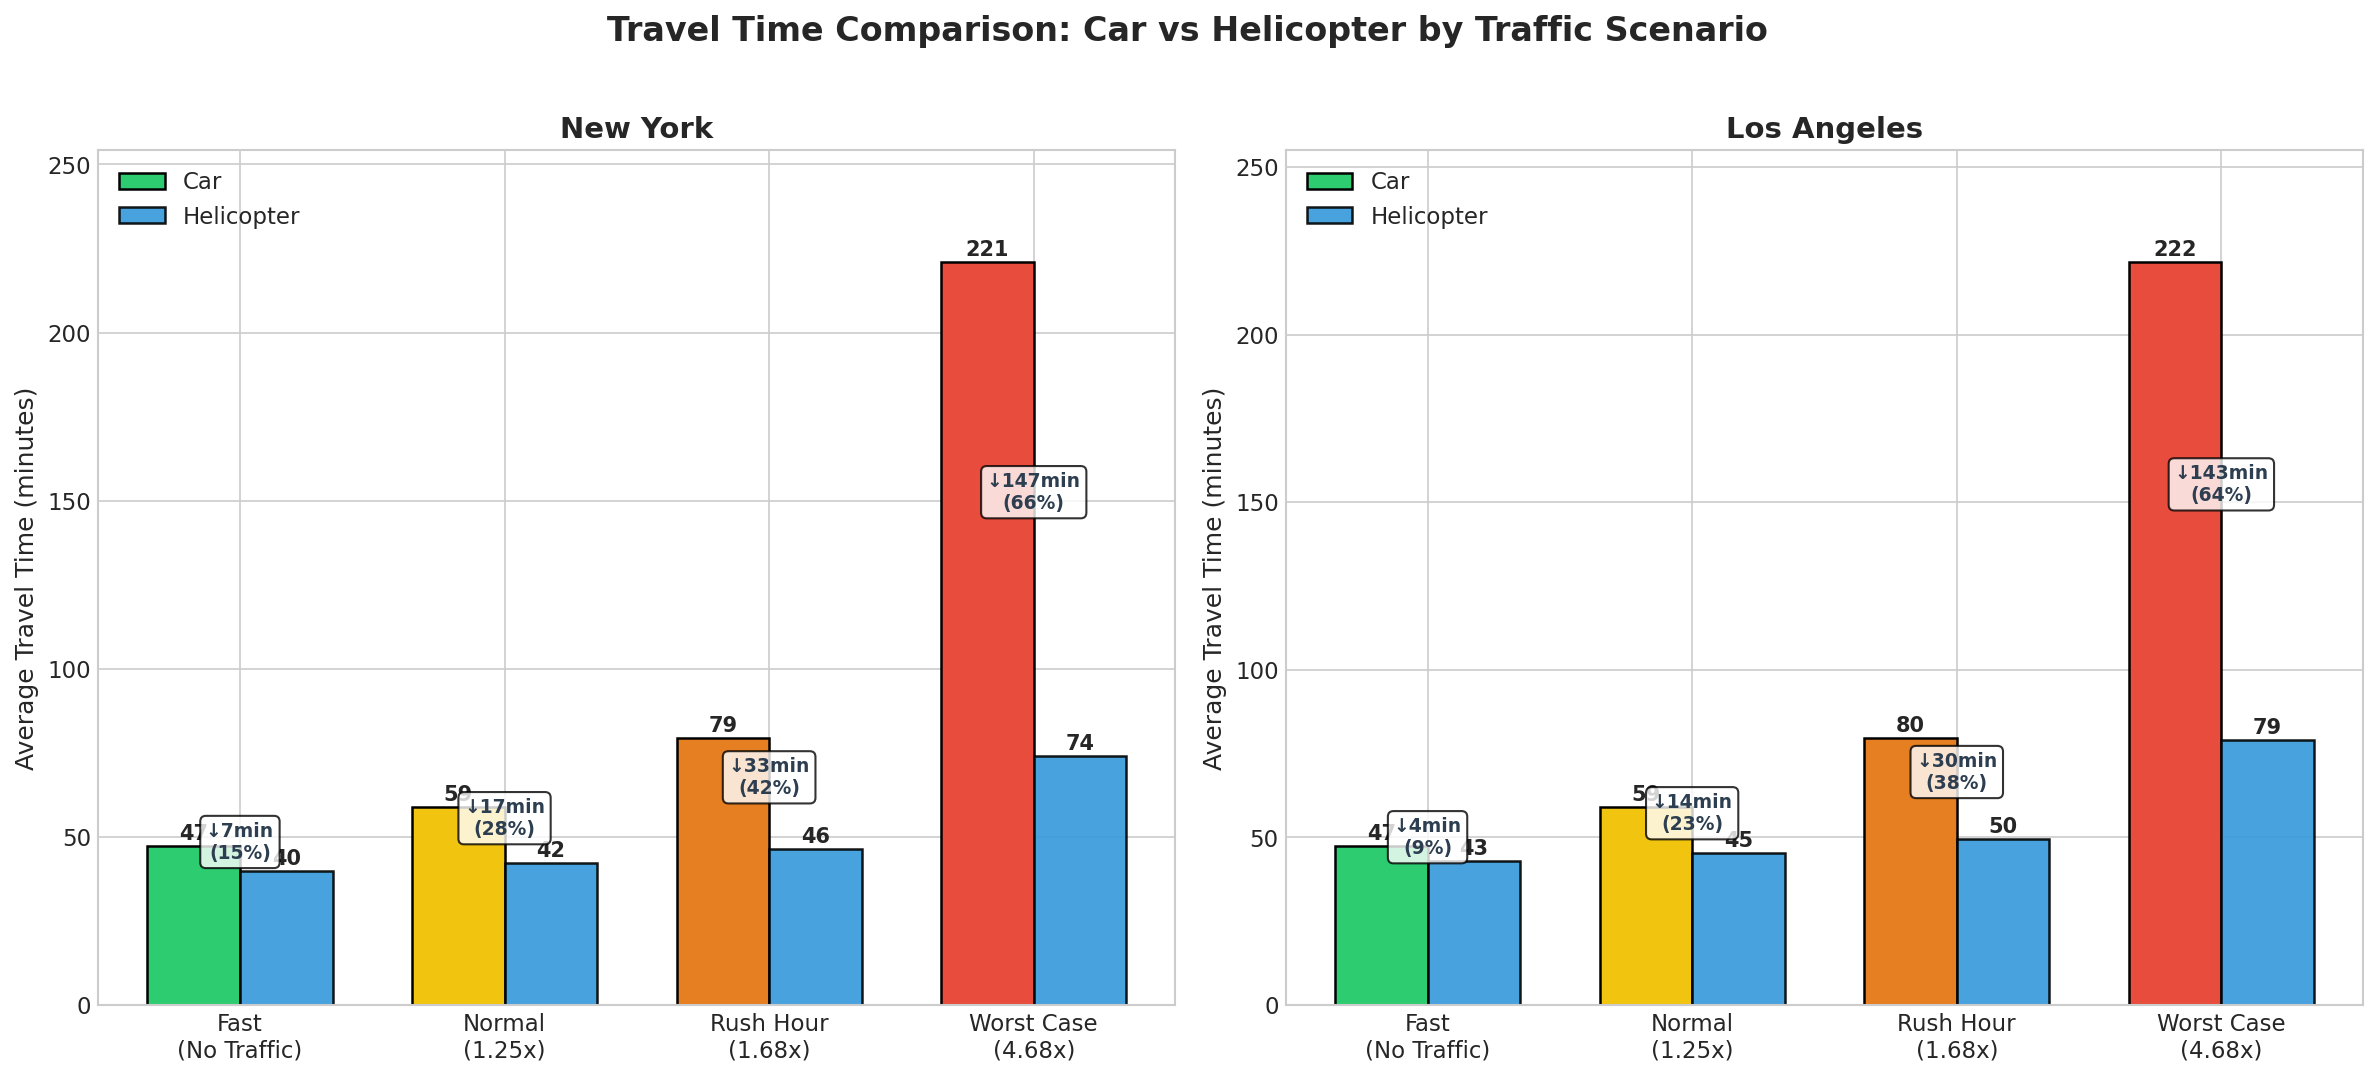
\includegraphics[width=0.88\textwidth,height=0.8\textheight,keepaspectratio]{../comparison_charts_en/fig1_scenario_comparison.png}
\end{center}
\end{frame}

\begin{frame}{Key Statistics}
\small
\begin{table}
\centering
\begin{tabular}{l|cccc|cccc}
\toprule
& \multicolumn{4}{c|}{\textcolor{revoBlue}{\textbf{New York}}} & \multicolumn{4}{c}{\textcolor{revoRed}{\textbf{Los Angeles}}} \\
\textbf{Metric} & Fast & Norm & Rush & Worst & Fast & Norm & Rush & Worst \\
\midrule
Car (min) & 47 & 59 & 79 & \textbf{221} & 47 & 59 & 80 & \textbf{222} \\
Heli (min) & 44 & 46 & 49 & \textbf{74} & 46 & 48 & 52 & \textbf{79} \\
\textcolor{revoGreen}{\textbf{Savings}} & \textcolor{revoGreen}{3} & \textcolor{revoGreen}{13} & \textcolor{revoGreen}{30} & \textcolor{revoGreen}{\textbf{147}} & \textcolor{revoGreen}{1} & \textcolor{revoGreen}{11} & \textcolor{revoGreen}{28} & \textcolor{revoGreen}{\textbf{143}} \\
\bottomrule
\end{tabular}
\end{table}

\vspace{0.5em}
\begin{center}
\large{\textcolor{revoGreen}{\textbf{Worst Case: Save 2+ Hours!}}}
\end{center}
\end{frame}

\begin{frame}{Speed Degradation by Scenario}
\begin{center}
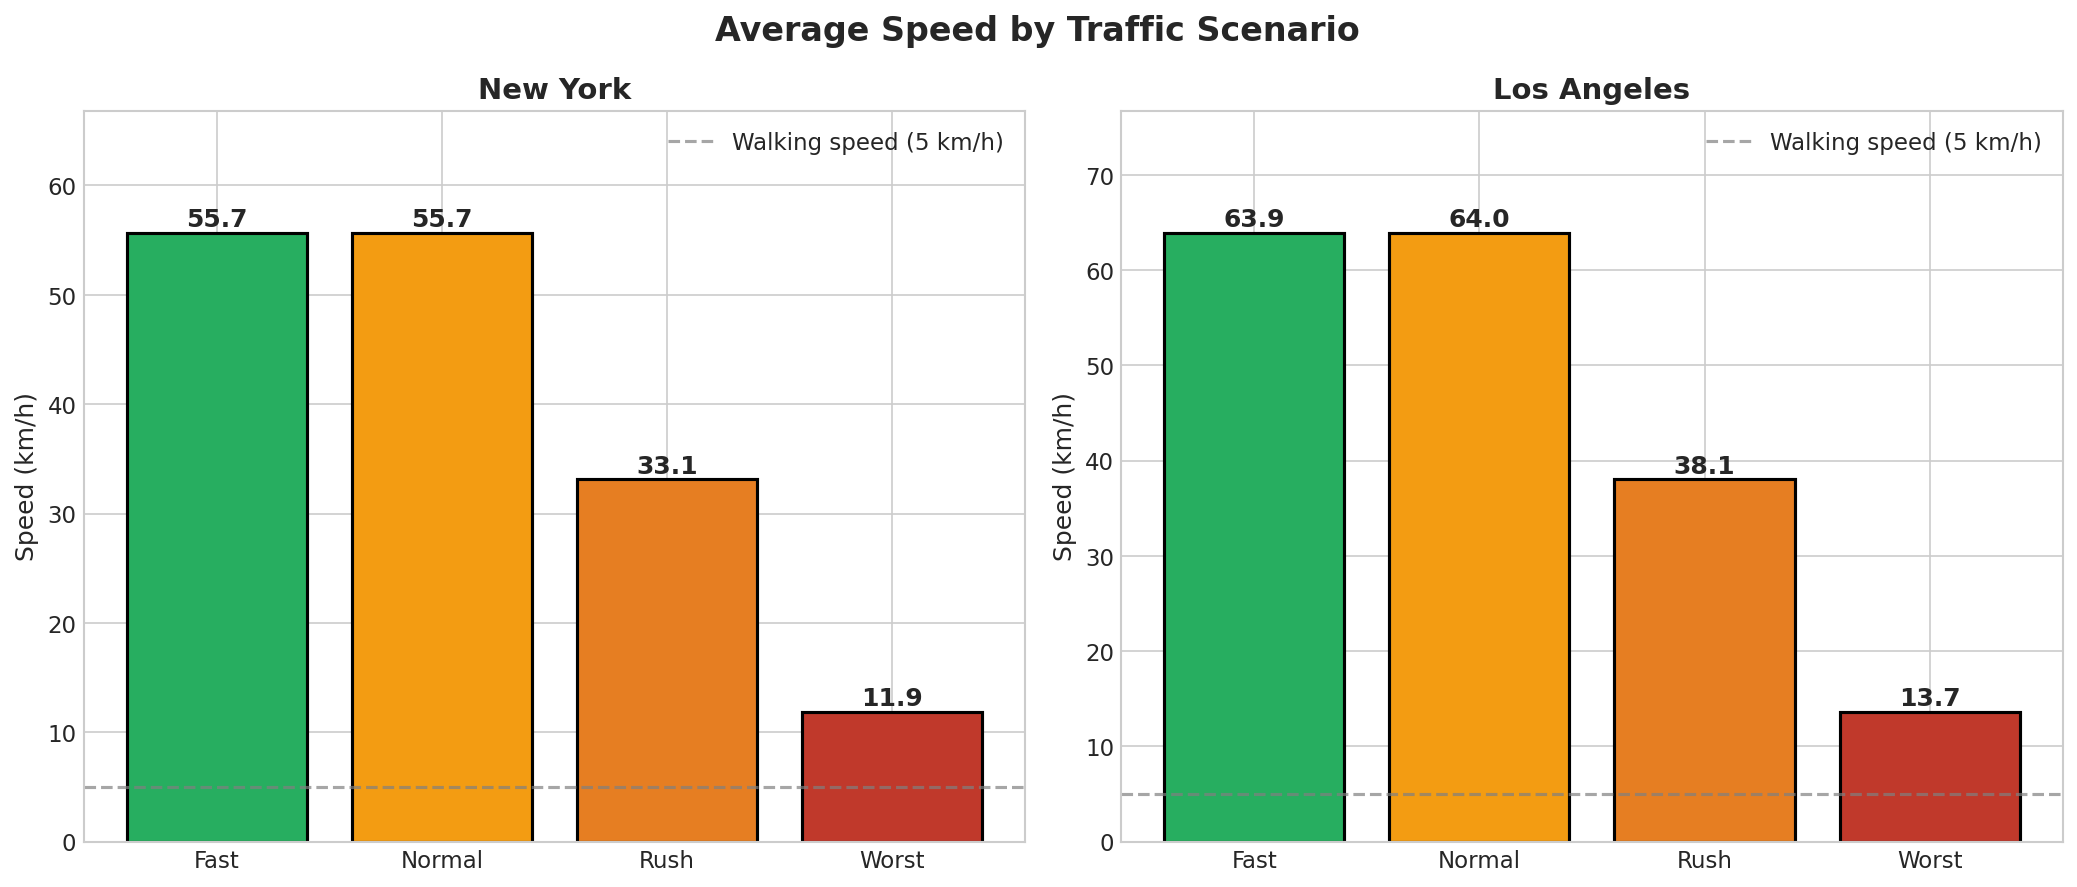
\includegraphics[width=0.85\textwidth,height=0.8\textheight,keepaspectratio]{../comparison_charts_en/fig2_speed_comparison.png}
\end{center}
\end{frame}

\begin{frame}{Time Savings Distribution}
\begin{center}
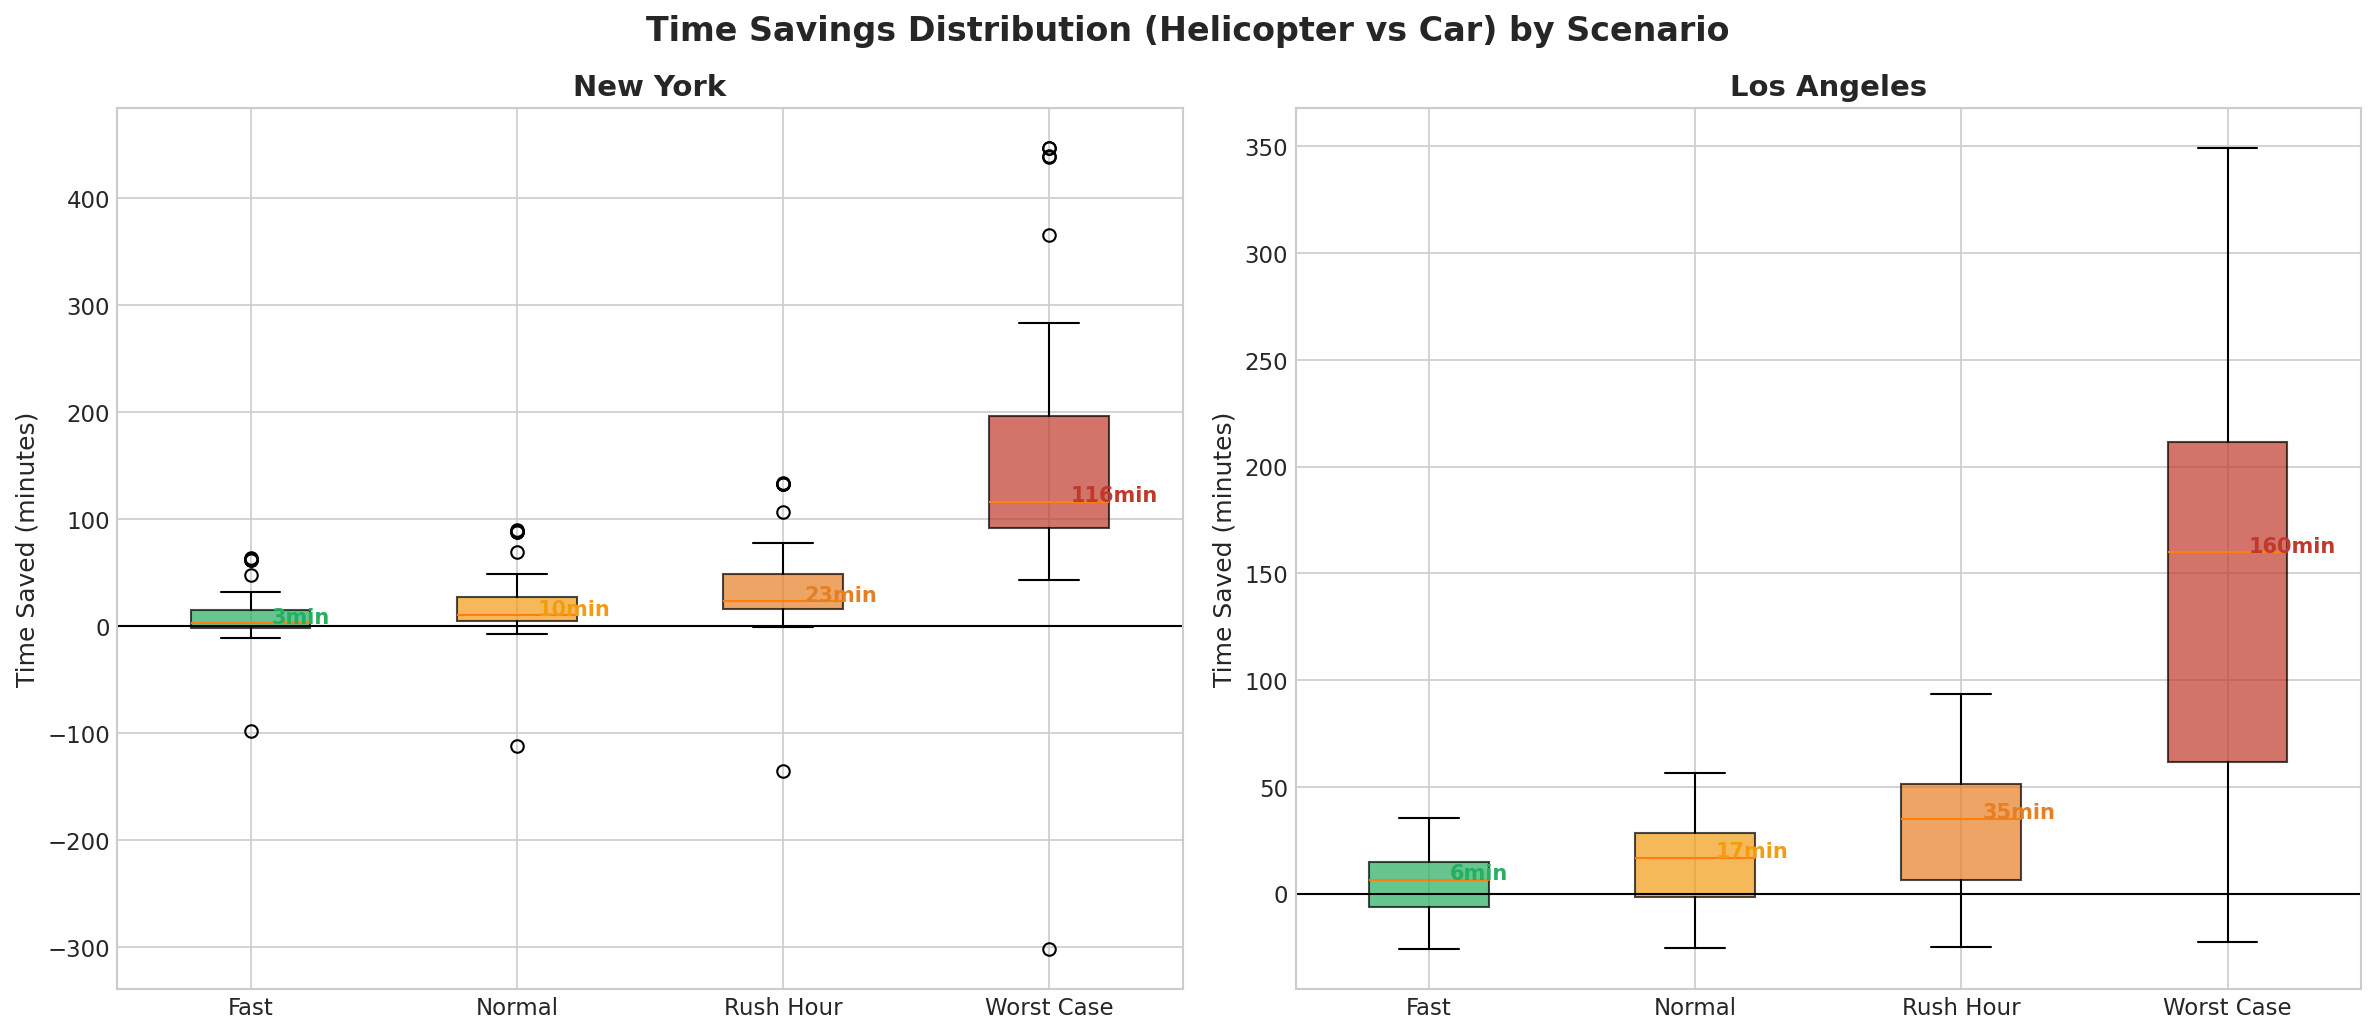
\includegraphics[width=0.88\textwidth,height=0.8\textheight,keepaspectratio]{../comparison_charts_en/fig4_savings_boxplot.png}
\end{center}
\end{frame}

\begin{frame}{Normal vs Worst Case: The Dramatic Difference}
\begin{center}
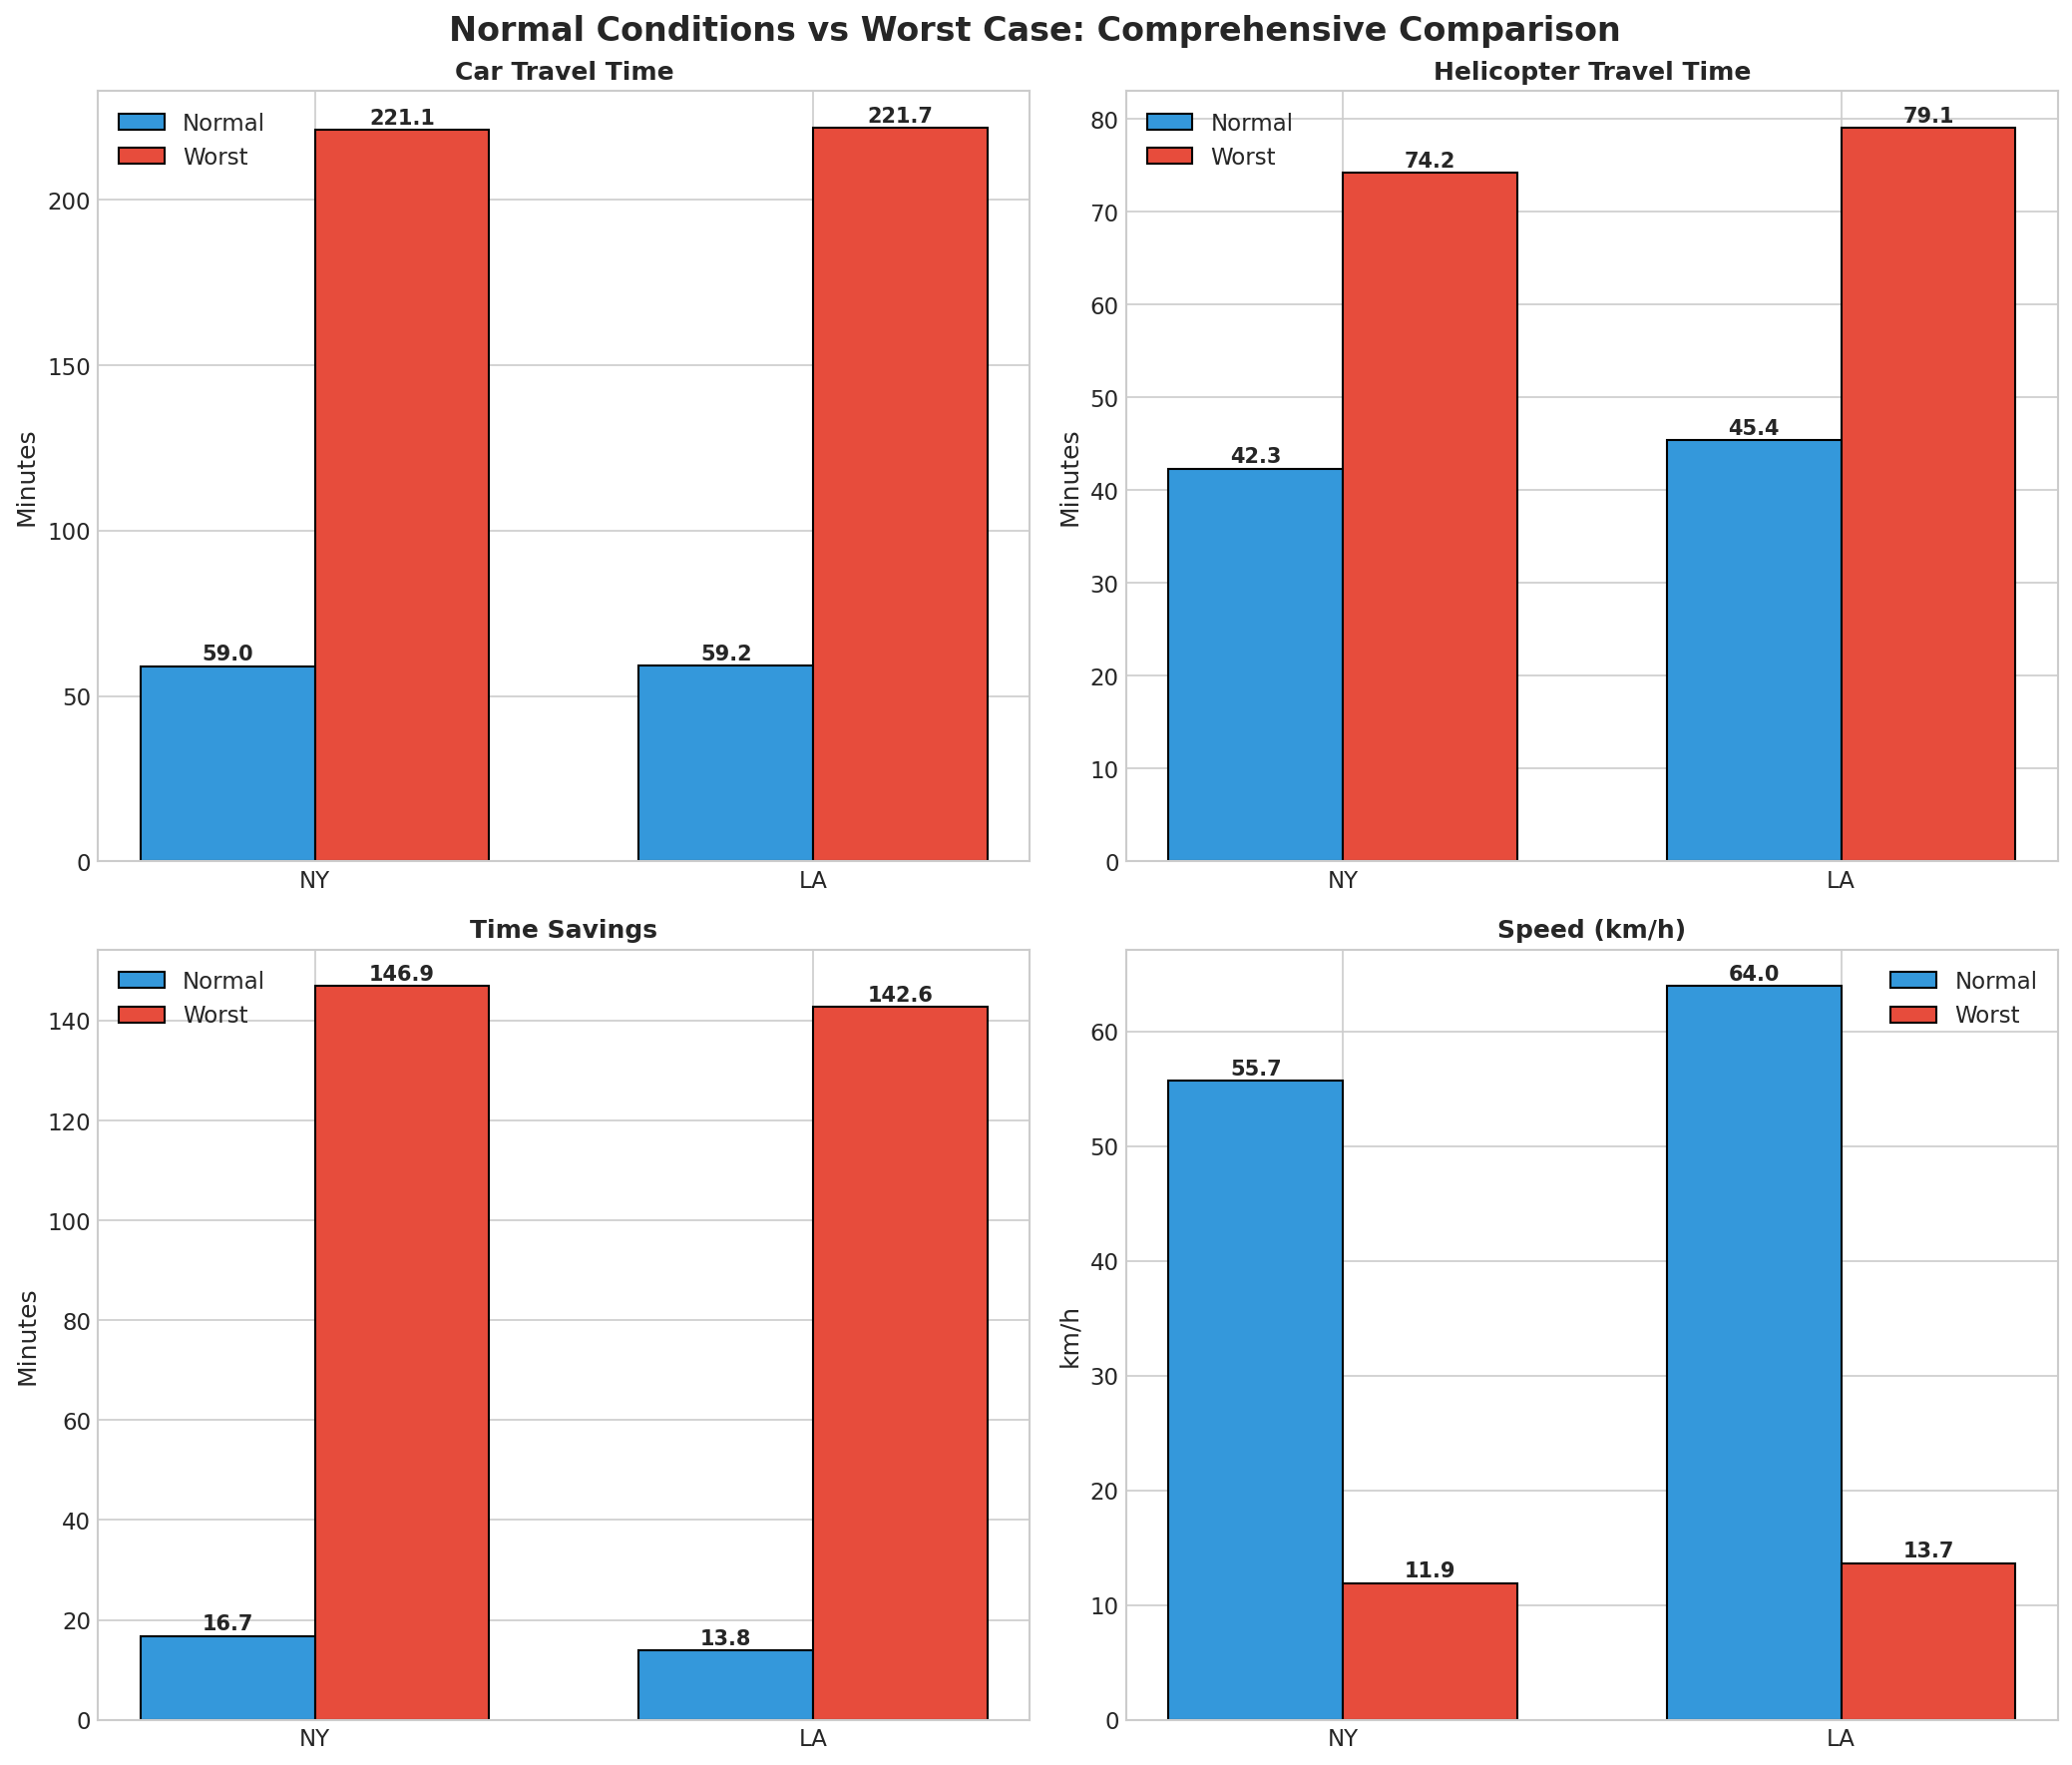
\includegraphics[width=0.82\textwidth,height=0.78\textheight,keepaspectratio]{../comparison_charts_en/fig6_normal_vs_worst.png}
\end{center}
\end{frame}

\begin{frame}{How Traffic Multiplies Travel Time}
\begin{center}
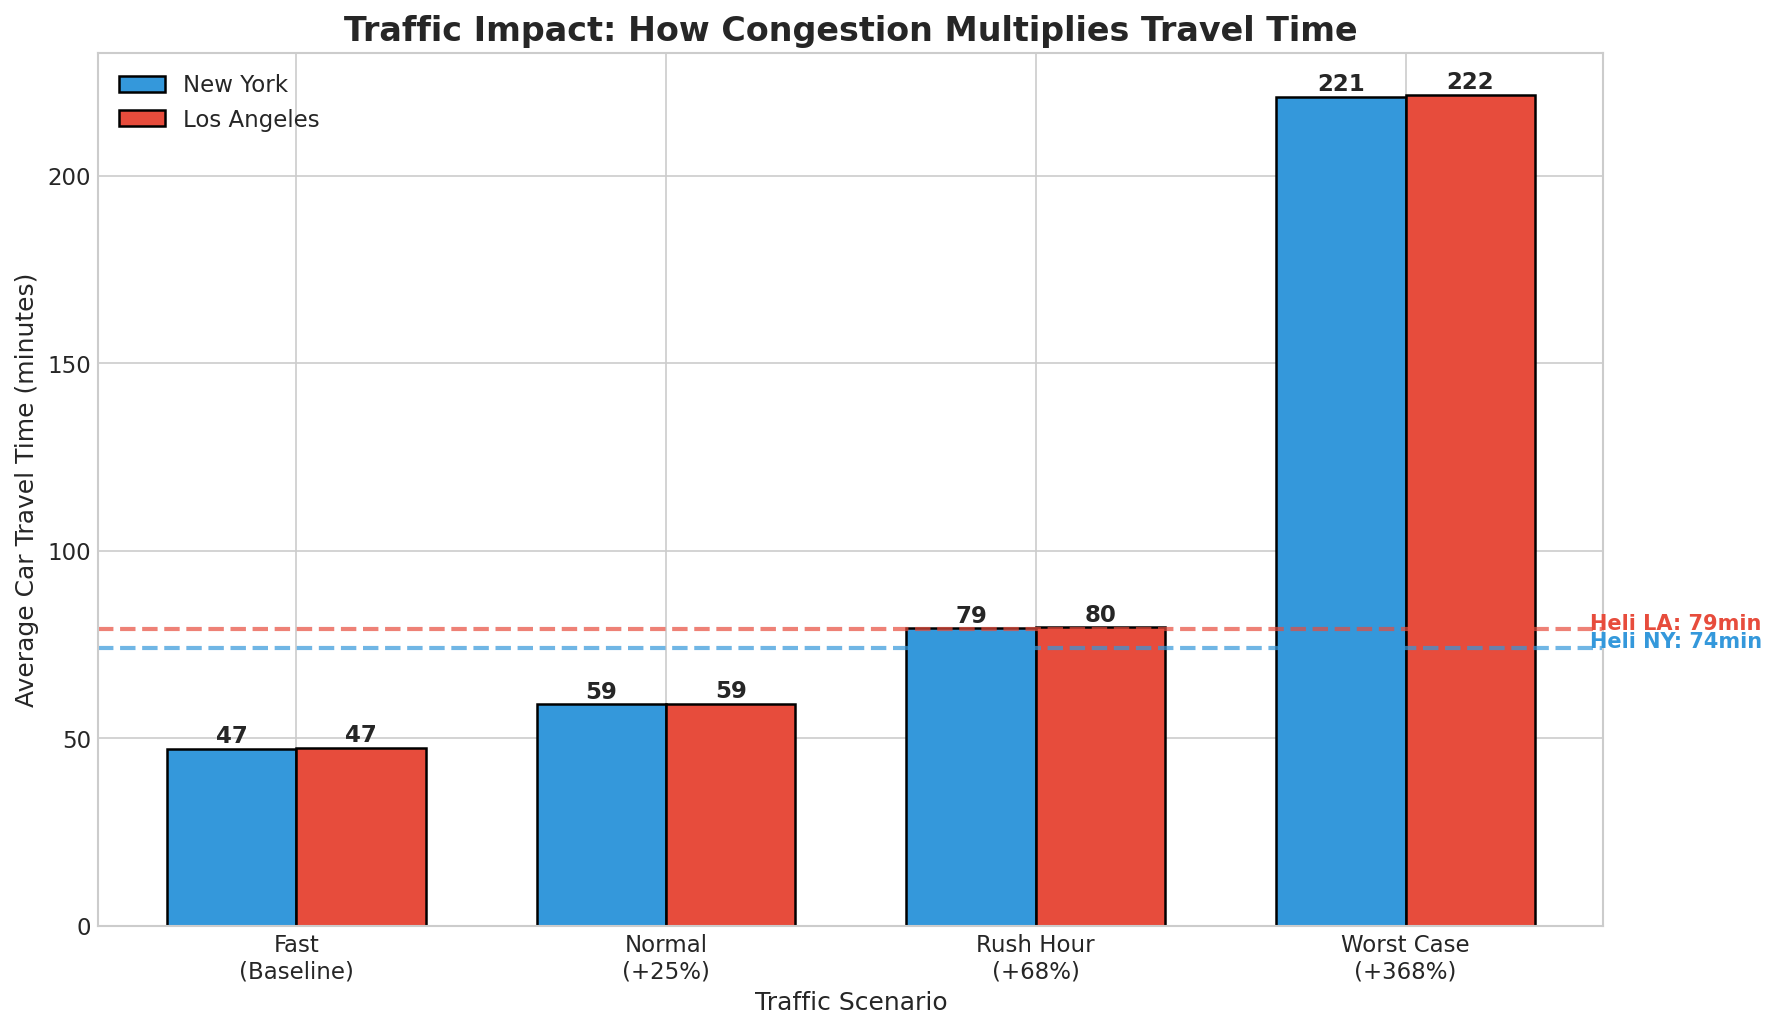
\includegraphics[width=0.85\textwidth,height=0.8\textheight,keepaspectratio]{../comparison_charts_en/fig5_multiplier_effect.png}
\end{center}
\end{frame}

\begin{frame}{Time per 100 Meters}
\begin{center}
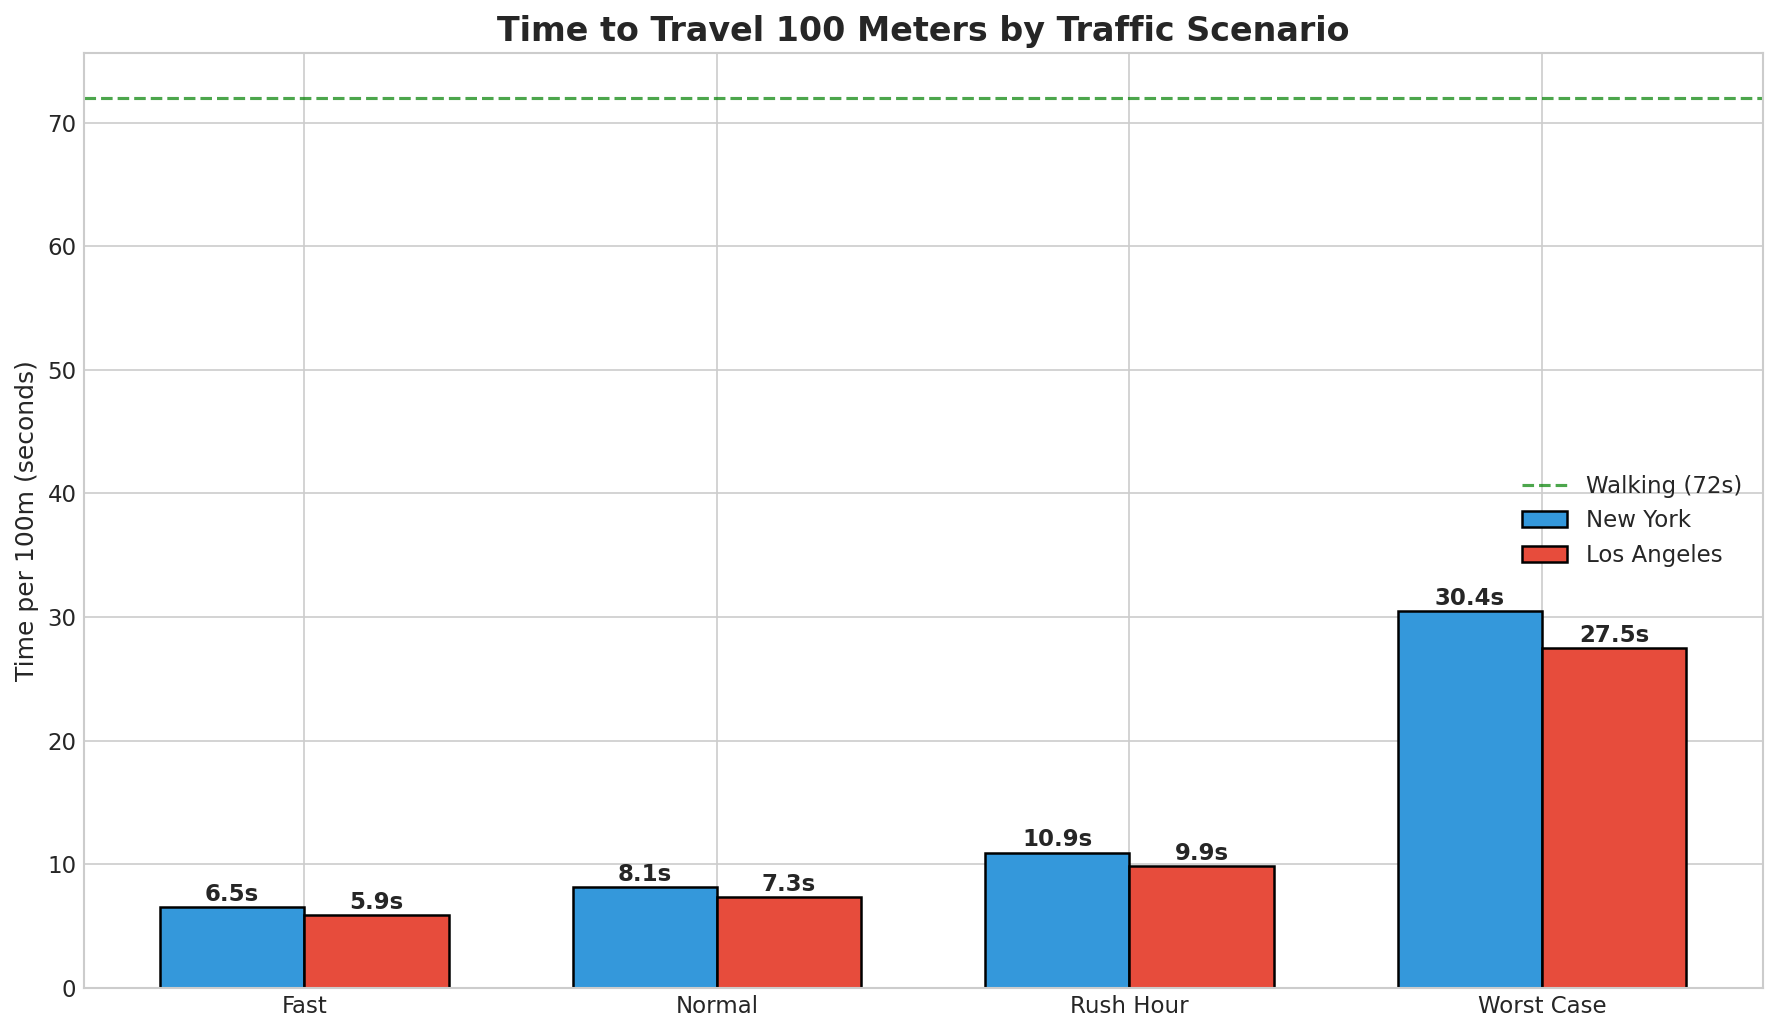
\includegraphics[width=0.8\textwidth,height=0.65\textheight,keepaspectratio]{../comparison_charts_en/fig3_time_100m.png}
\end{center}

\vspace{0.3em}
\begin{columns}
\column{0.5\textwidth}
\begin{center}
\small{\textbf{Worst Case:} 30 sec / 100m}
\end{center}

\column{0.5\textwidth}
\begin{center}
\small{\textbf{Walking:} 72 sec / 100m}
\end{center}
\end{columns}
\end{frame}

\begin{frame}{Time Breakdown: Worst Case}
\begin{center}
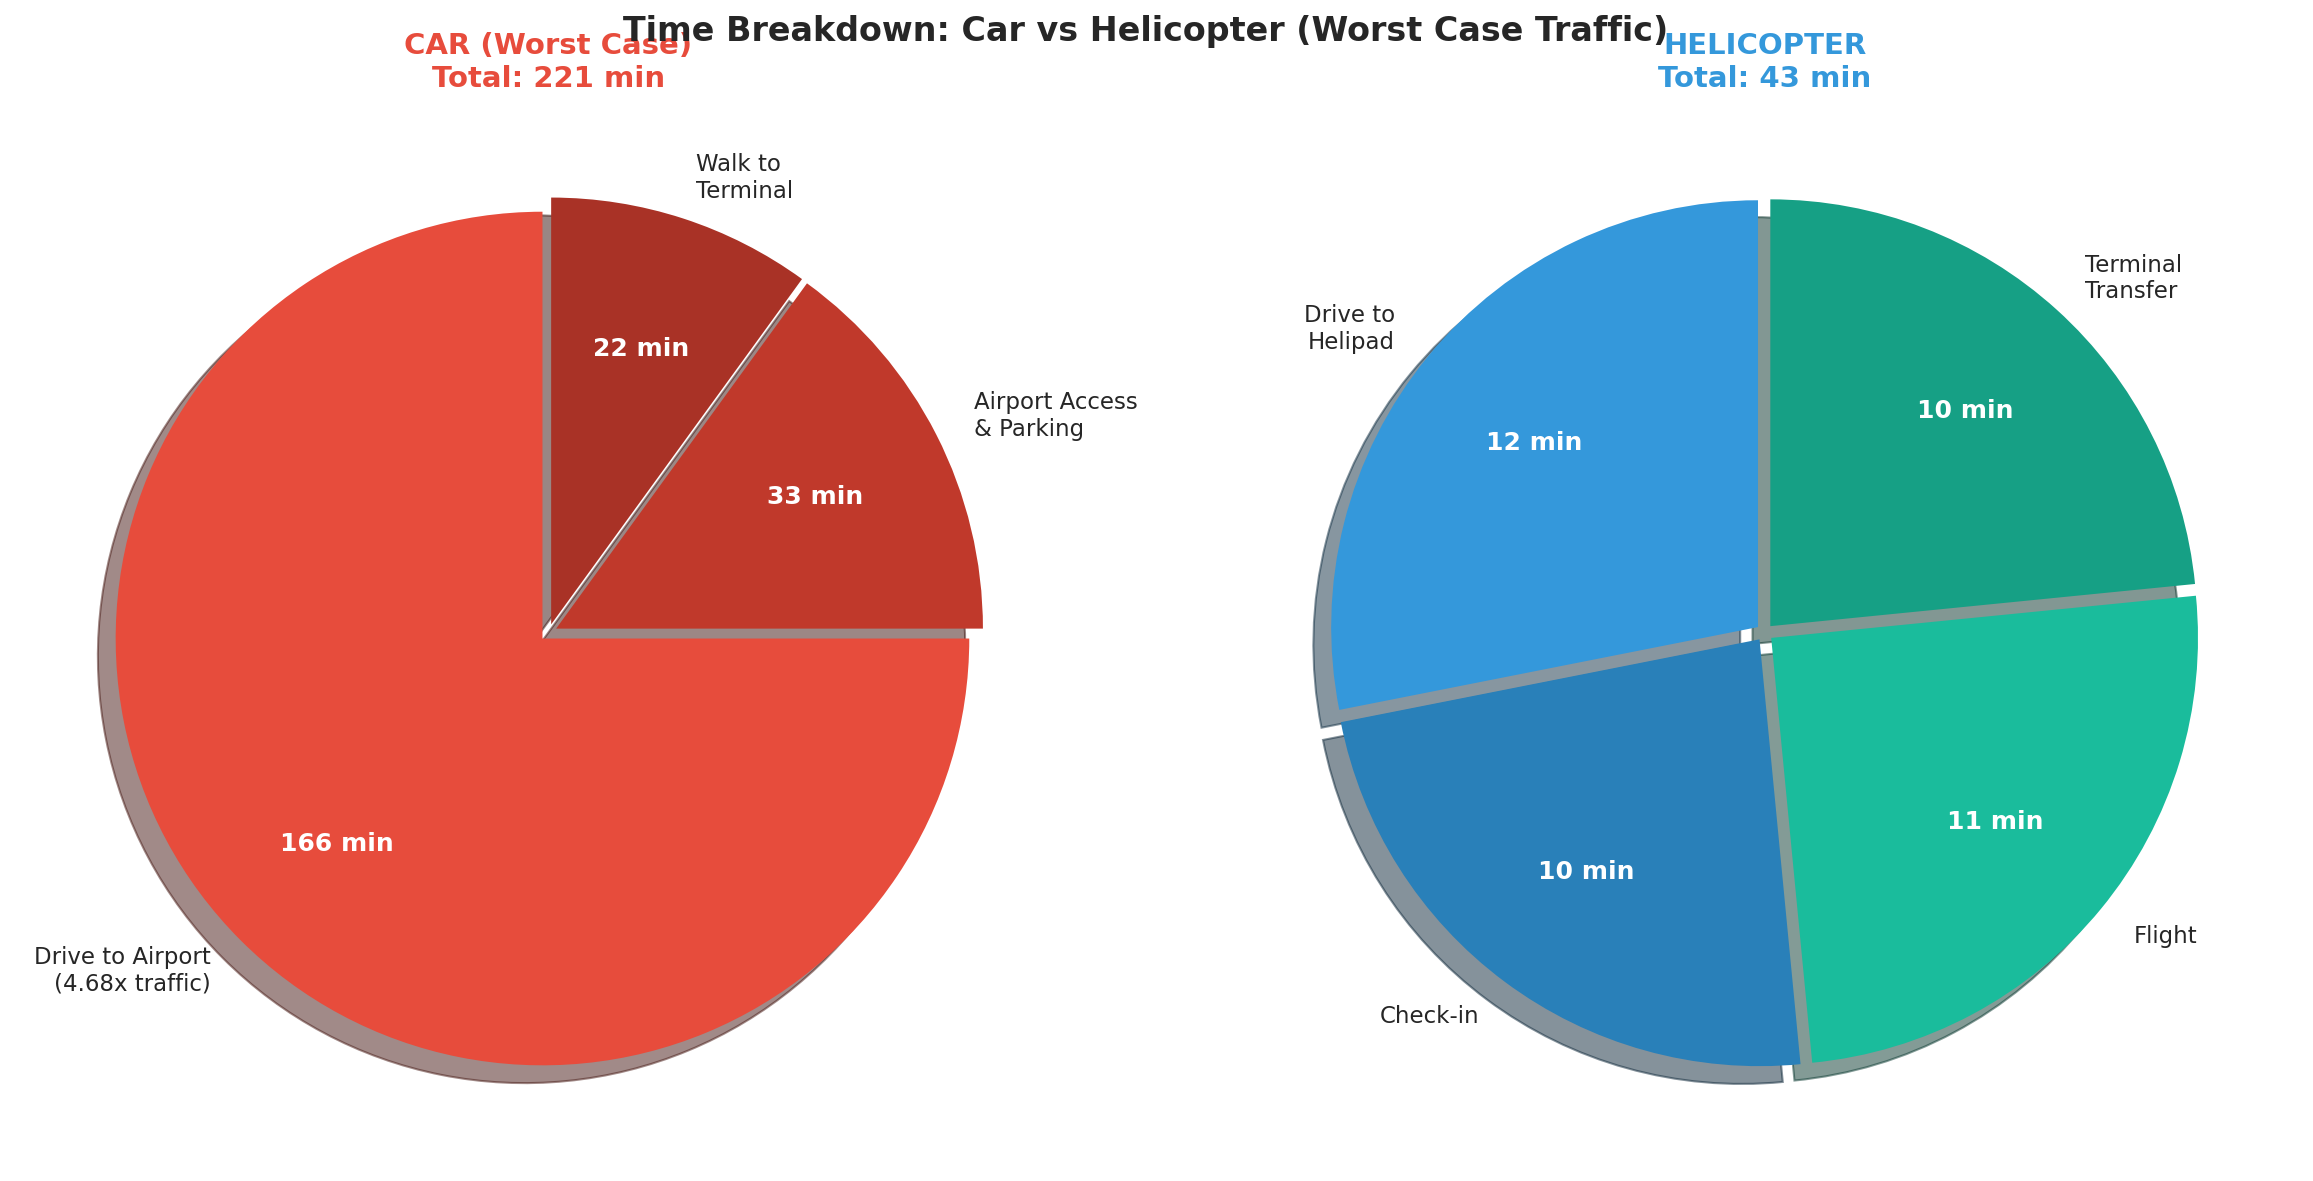
\includegraphics[width=0.75\textwidth,height=0.78\textheight,keepaspectratio]{../diagrams/time_breakdown_en.png}
\end{center}
\end{frame}

\begin{frame}{Savings Distribution Histogram}
\begin{center}
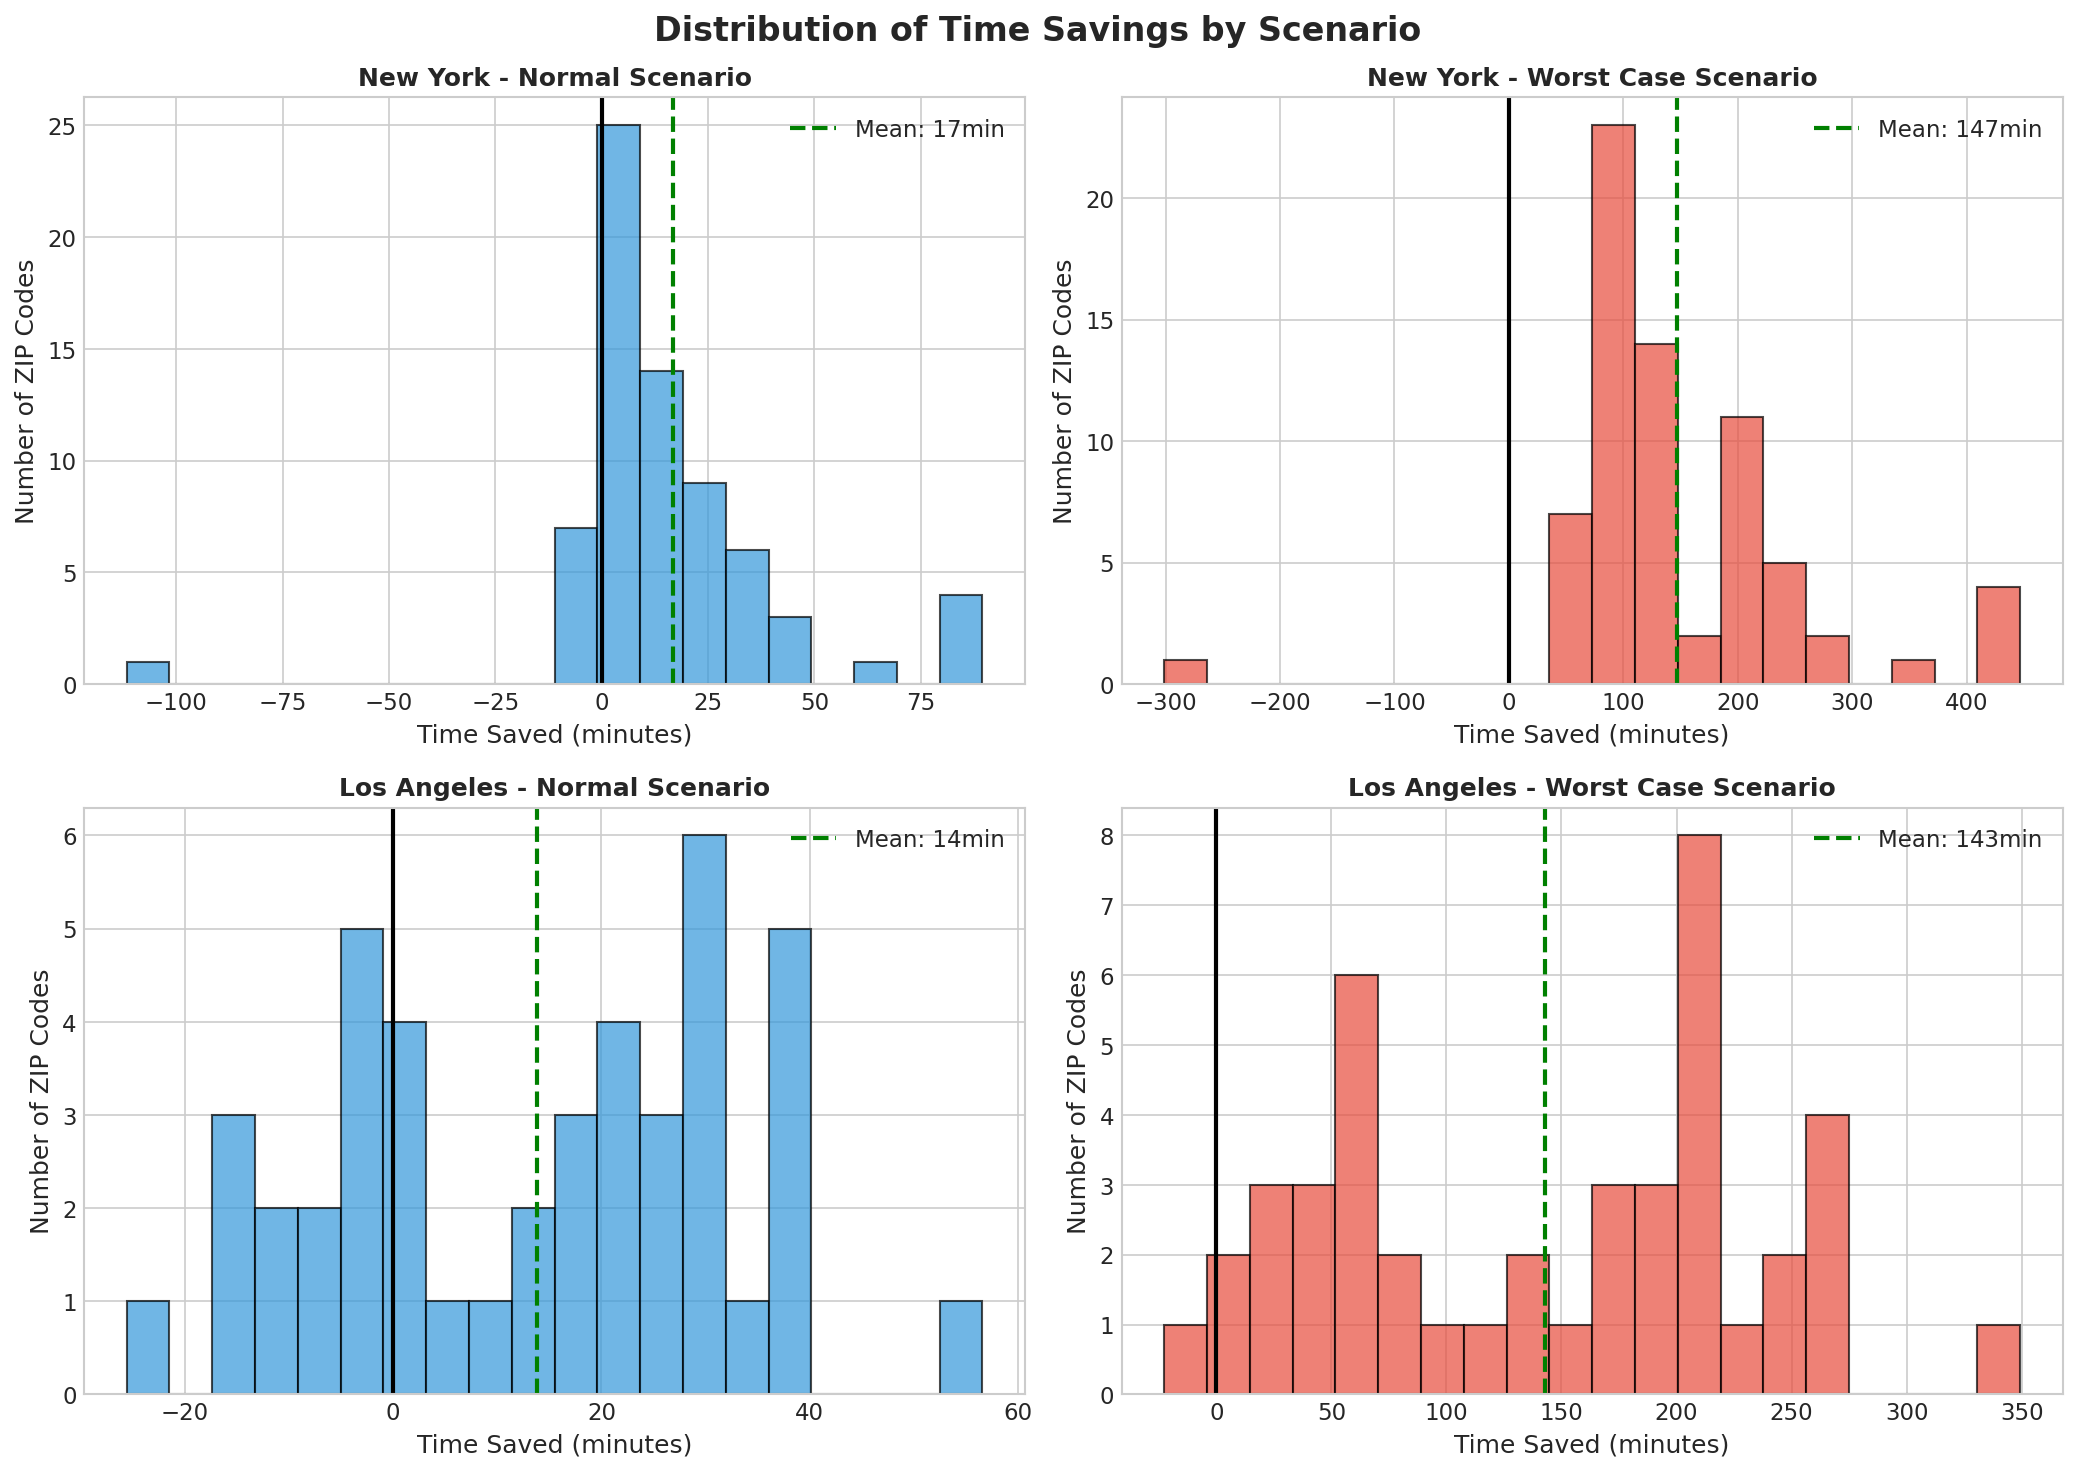
\includegraphics[width=0.85\textwidth,height=0.78\textheight,keepaspectratio]{../comparison_charts_en/fig8_savings_histogram.png}
\end{center}
\end{frame}

% ============================================================================
\section{Key Insights}
% ============================================================================

\begin{frame}{Why Helicopter Wins in Worst Case}
\begin{columns}
\column{0.5\textwidth}
\begin{block}{\faCarSide\ Car Travel}
\begin{itemize}
    \item \textcolor{revoRed}{\textbf{100\%}} affected by traffic
    \item Time increases \textcolor{revoRed}{\textbf{4.68x}}
    \item Unpredictable delays
    \item Stress and fatigue
\end{itemize}
\end{block}

\column{0.5\textwidth}
\begin{block}{\faHelicopter\ Helicopter Travel}
\begin{itemize}
    \item Only \textcolor{revoGreen}{\textbf{20\%}} affected by traffic
    \item Time increases only \textcolor{revoGreen}{\textbf{1.6x}}
    \item Predictable schedule
    \item Comfort and productivity
\end{itemize}
\end{block}
\end{columns}

\vspace{0.5em}
\begin{center}
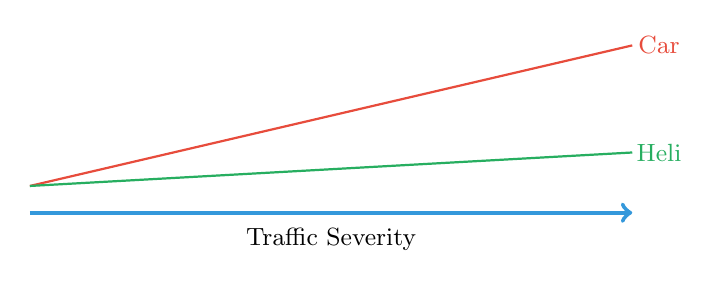
\begin{tikzpicture}[scale=0.85]
    \draw[ultra thick, ->, revoBlue] (0,0) -- (9,0);
    \node at (4.5,-0.4) {\small Traffic Severity};
    \draw[thick, revoRed] (0,0.4) -- (9,2.5);
    \node[revoRed] at (9.4,2.5) {\small Car};
    \draw[thick, revoGreen] (0,0.4) -- (9,0.9);
    \node[revoGreen] at (9.4,0.9) {\small Heli};
\end{tikzpicture}
\end{center}
\end{frame}

\begin{frame}{Business Value Proposition}
\begin{columns}
\column{0.33\textwidth}
\begin{center}
\textcolor{revoBlue}{\Large{\faClock}}\\[0.3em]
\small{\textbf{Time Savings}}\\[0.3em]
\large{147 min}\\
\footnotesize{(NY worst case)}
\end{center}

\column{0.33\textwidth}
\begin{center}
\textcolor{revoGreen}{\Large{\faCheckCircle}}\\[0.3em]
\small{\textbf{Reliability}}\\[0.3em]
\large{99\%}\\
\footnotesize{advantage rate}
\end{center}

\column{0.33\textwidth}
\begin{center}
\textcolor{revoOrange}{\Large{\faPlane}}\\[0.3em]
\small{\textbf{Never Miss}}\\[0.3em]
\large{Flights}\\
\footnotesize{predictable arrival}
\end{center}
\end{columns}

\vspace{0.8em}
\begin{exampleblock}{ROI Consideration}
\small{2+ hours saved = productive meeting time, reduced stress, guaranteed connections}
\end{exampleblock}
\end{frame}

% ============================================================================
\section{Conclusions}
% ============================================================================

\begin{frame}{Summary of Findings}
\begin{columns}
\column{0.5\textwidth}
\begin{block}{\textcolor{revoBlue}{New York}}
\begin{itemize}
    \item 70 ZIP codes analyzed
    \item 27 Manhattan locations
    \item \textbf{147 min} worst case savings
    \item \textbf{66\%} time reduction
    \item 99\% show helicopter advantage
\end{itemize}
\end{block}

\column{0.5\textwidth}
\begin{block}{\textcolor{revoRed}{Los Angeles}}
\begin{itemize}
    \item 44 ZIP codes analyzed
    \item Distributed coverage
    \item \textbf{143 min} worst case savings
    \item \textbf{64\%} time reduction
    \item 98\% show helicopter advantage
\end{itemize}
\end{block}
\end{columns}

\vspace{0.5em}
\begin{alertblock}{Key Takeaway}
\centering
\small{The worse the traffic, the greater the helicopter advantage.\\
In extreme conditions, helicopter is the \textbf{only viable option} for time-sensitive travel.}
\end{alertblock}
\end{frame}

\begin{frame}{Complete Summary Statistics}
\begin{center}
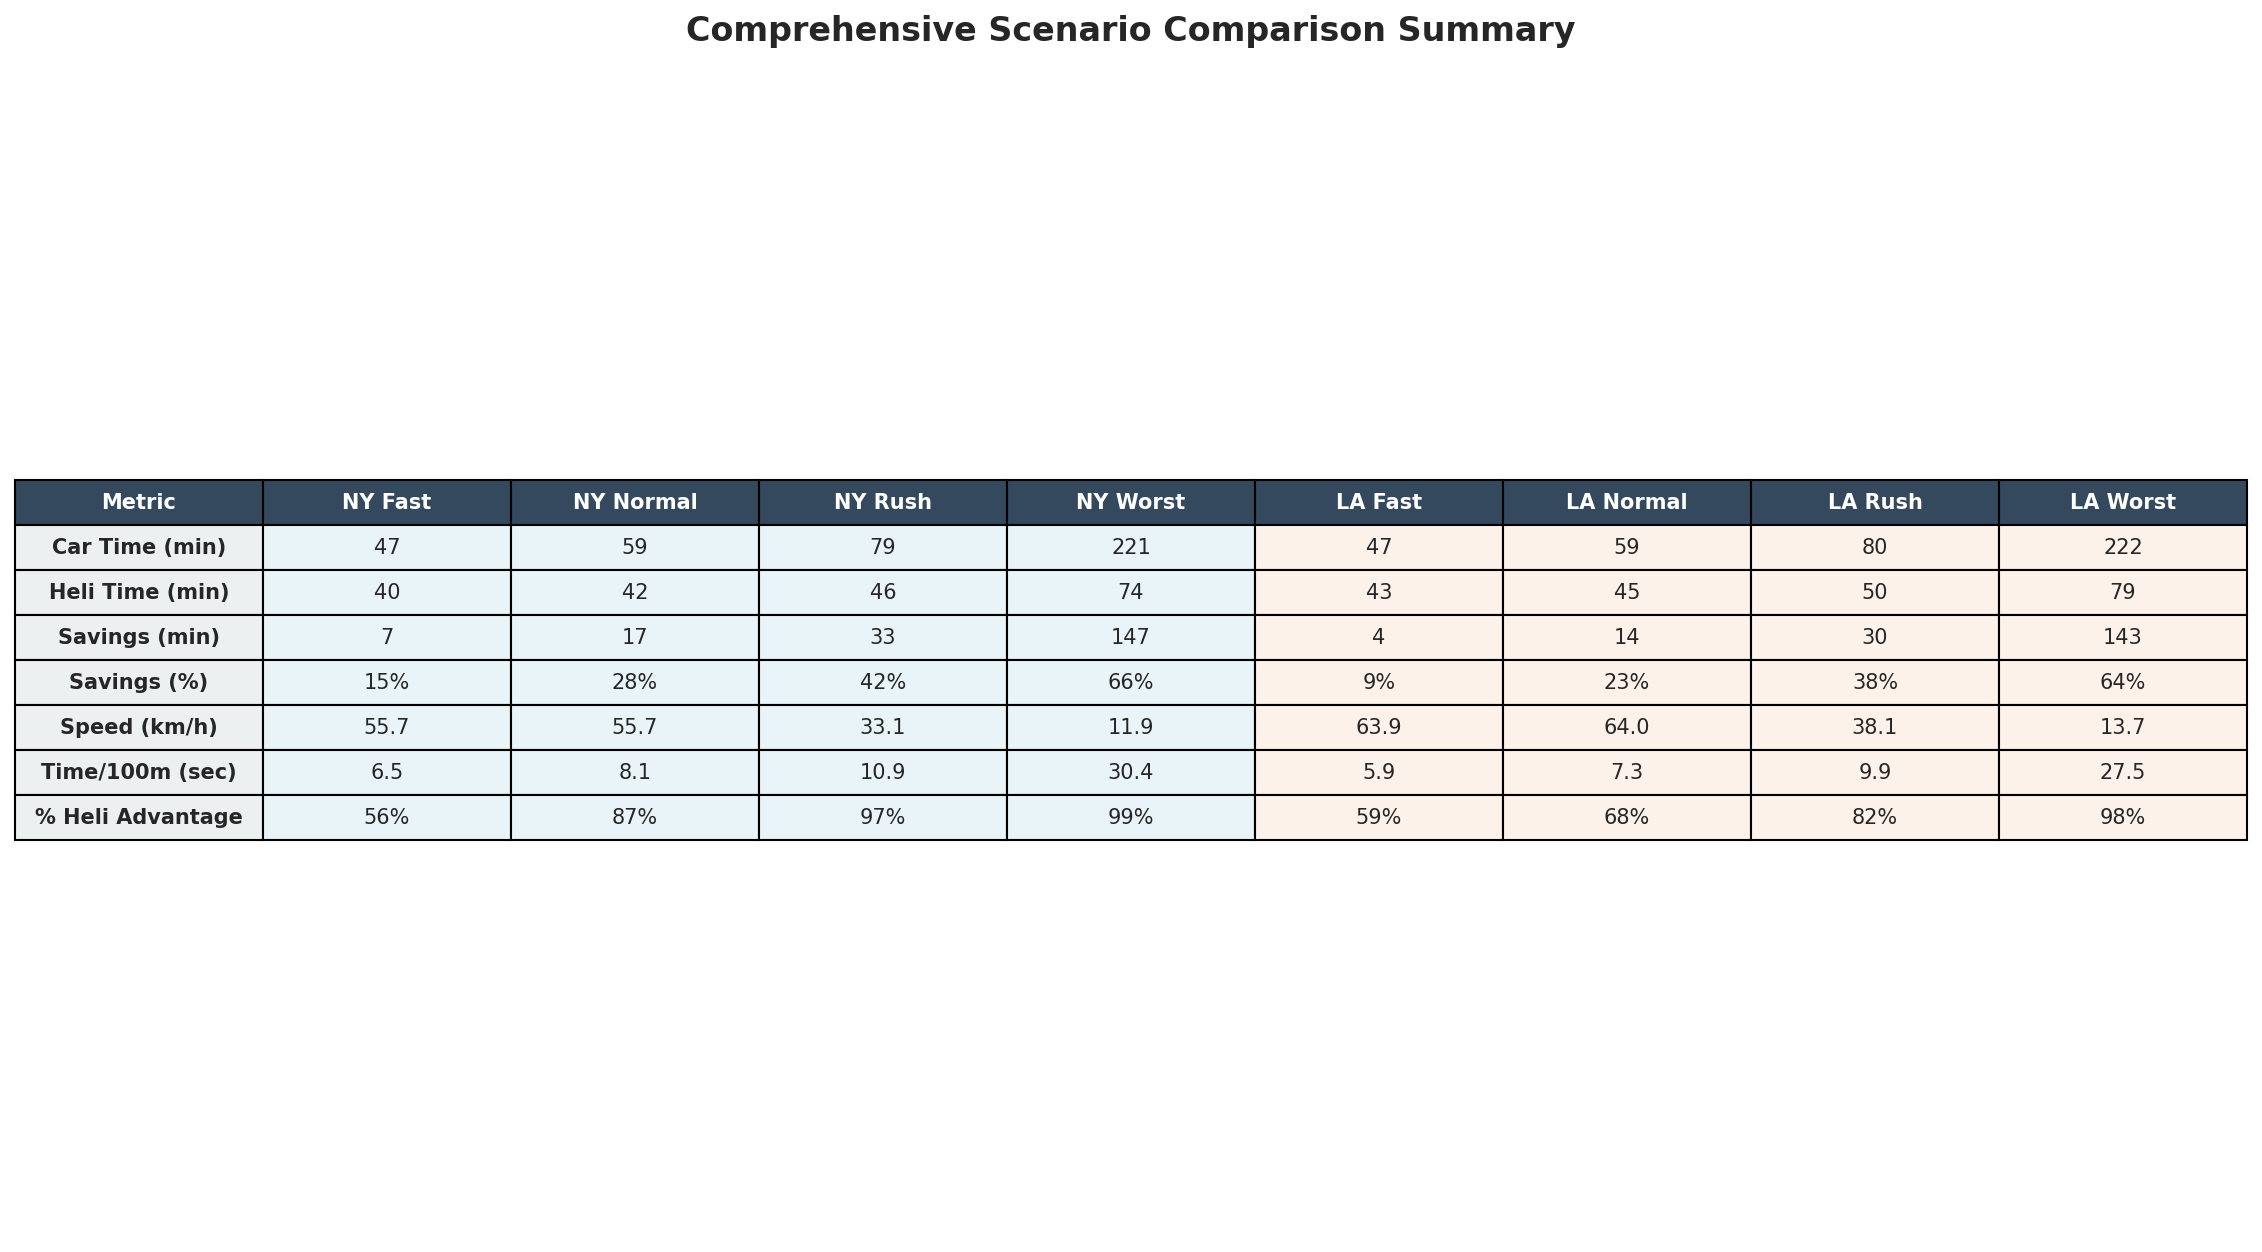
\includegraphics[width=0.88\textwidth,height=0.78\textheight,keepaspectratio]{../comparison_charts_en/fig7_summary_table.png}
\end{center}
\end{frame}

\begin{frame}
\begin{center}
\Huge{\textbf{Thank You}}\\[1.5em]
\Large{Questions?}\\[1.5em]
\normalsize{REVO Helicopter Services}\\
\small{\textit{Strategic Analysis Division}}\\[0.8em]
\small{December 2025}
\end{center}
\end{frame}

\end{document}
